\documentclass[20pt]{article}
\usepackage{fullpage}
\usepackage{graphicx}
\usepackage{color}
\usepackage[utf8]{inputenc}
\usepackage[spanish]{babel}
\usepackage{enumerate}

\begin{document}

\begin{center}
	\begin{huge}
		\textbf{Cinema}\\
	\end{huge}
\end{center}

\begin{center}
	\begin{huge}
		\textbf{Manual de usuario}\\ 
	\end{huge}
\end{center}



\begin{large}
	\textbf{1:Inicio de sesión}\\\\
\end{large}

\begin{center}
	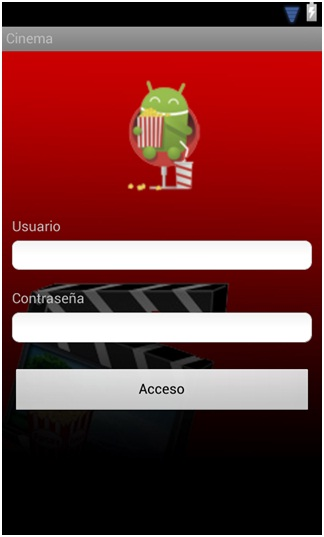
\includegraphics[totalheight=1.8in,width=1.4in]{inicio}\\
\end{center}
Al iniciar la aplicación se presentara esta pantalla que representa el inicio de sesión. En el primer cuadro de texto se ingresa el usuario registrado en el cine. En el segundo cuadro se ingresa la contraseña, que es el numero de cedula perteneciente al usuario. Una vez ingresados ambos campos se podrá acceder al sistema.\\\\\



\begin{large}
	\textbf{2:Menu principal}\\\\
\end{large}
\begin{center}
	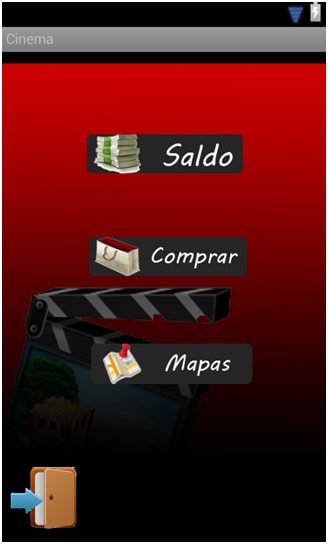
\includegraphics[totalheight=1.8in,width=1.4in]{menu_principal}\\
\end{center}

En el menú principal se mostraran cuatro opciones: 

\begin{itemize}
	\item Saldo: aquí se muestra el saldo disponible en la cuenta.
	\item Comprar: se catalogan las ventas que ofrece el cine para el usuario.
	\item Mapas: se muestran las ubicaciones geográficas de los distintos locales del cine dentro de la ciudad.
	\item Cerrar sesión.\\\\
\end{itemize}



\begin{large}
	\textbf{3:Saldo disponible}\\\
\end{large}
\begin{center}
	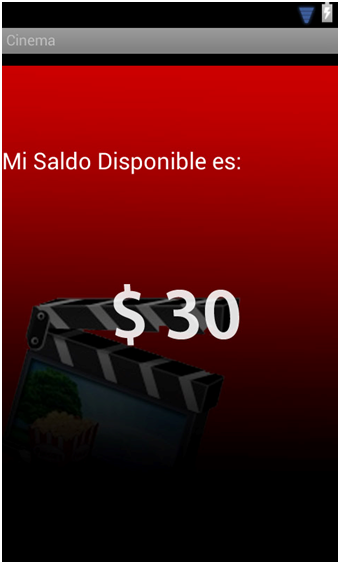
\includegraphics[totalheight=1.8in,width=1.4in]{saldo_disponible}
\end{center}
Se muestra el saldo disponible en la cuenta del usuario.
Para regresar al menú principal, se presiona el botón “deshacer” del Smartphone.\\\\\\

\begin{large}
	\textbf{4:Comprar}\\\
\end{large}

\begin{enumerate}[(a)]
	\item Seleccion de cine\\Al seleccionar en el menú principal “Comprar”, el usuario debe de seleccionar en que cine se 	encuentra para seguir con el debido procedimiento de la compra.\\
	
	\begin{center}
		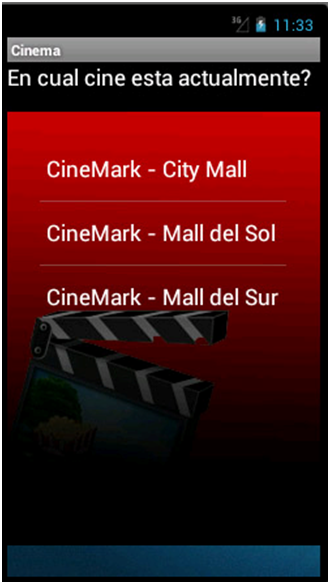
\includegraphics[totalheight=1.8in,width=1.4in]{seleccion_de_cine}
	\end{center}



	\item Datos de factura\\
	Se ingresa el código de la factura que viene impreso en el ticket, como se indica en la figura.
	Mediante este código se obtiene la función, el asiento, la sala y los datos personales del usuario necesarios para 			que el cine facture la compra.\\

\begin{center}
	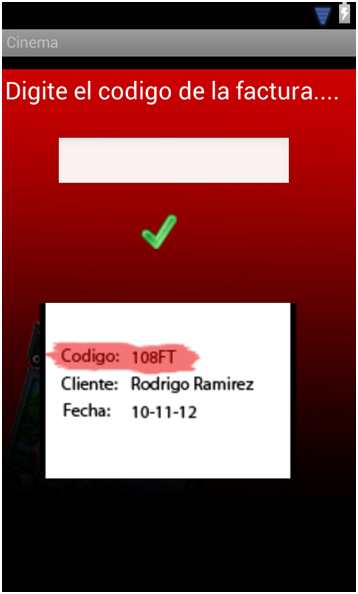
\includegraphics[totalheight=1.8in,width=1.4in]{datos_de_factura}
\end{center}



\item Menu de compra\\
\begin{center}
	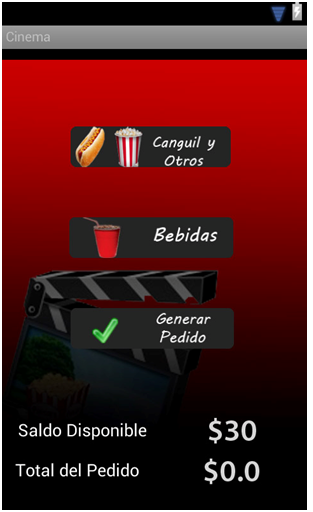
\includegraphics[totalheight=1.8in,width=1.4in]{menu_de_compra}
\end{center}

En el menú principal se mostraran dos opciones: 
\begin{itemize}
\item Canguil y otros: se muestran los snacks. 
\item Bebidas: se muestran las bebidas con sus tamaños.
\end{itemize}

Una vez que se seleccionan las compras, se oprime generar pedido y se genera la factura. Adicionalmente se muestran el saldo disponible en cada momento y el total del pedido.\\\\

\item Canguil y otros
Se muestran los distintos snacks que ofrece el cine. Se debe seleccionar solo uno por compra. Para hacer esto, se presiona uno de los iconos mostrados y luego se oprime el visto verde para aceptar la compra.\\\\
\begin{center}
	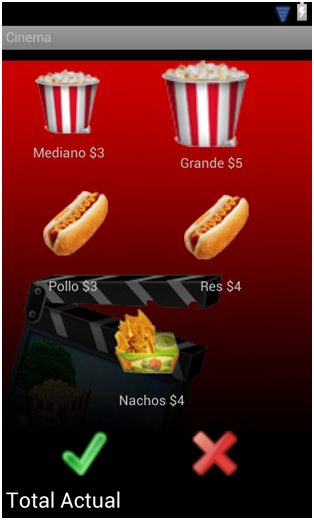
\includegraphics[totalheight=1.8in,width=1.4in]{canguil_y_otros}
\end{center}

\item Bebidas
Se selecciona la marca de la bebida en el combo box. Para seleccionar el tamaño se presiona sobre el icono mostrado. Para aceptar la compra se oprime el visto verde. Caso contrario, si quiere cancelar la compra, se presiona la cruz. En el total actual se muestra el total de la compra. Una vez que oprime alguno de estos botones, la aplicación regresa a Menú Compra.
\begin{center}
	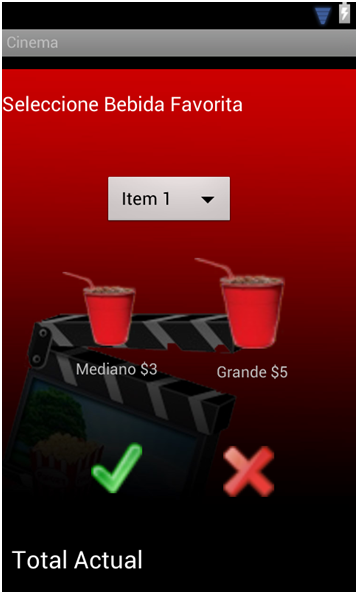
\includegraphics[totalheight=1.8in,width=1.4in]{bebidas}
\end{center}


\item Generar pedido
Al seleccionar en el menú de compra “generar pedido”, se genera la factura con la información ingresada anteriormente.\\
\begin{center}
	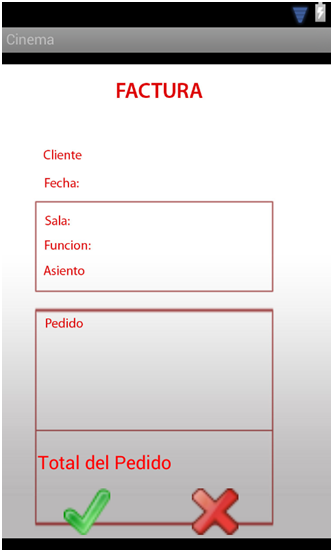
\includegraphics[totalheight=1.8in,width=1.4in]{generar_pedido}
\end{center}


\end{enumerate}


\begin{large}
\textbf{5:Mapas}\\\
\end{large}
Se muestran las localidades en Guayaquil de los cines en los que se puede utilizar esta aplicación. Una vez que se presiona uno de estos, nos da la referencia de la ubicación geográfica con respecto a donde nos encontramos.
\begin{center}
	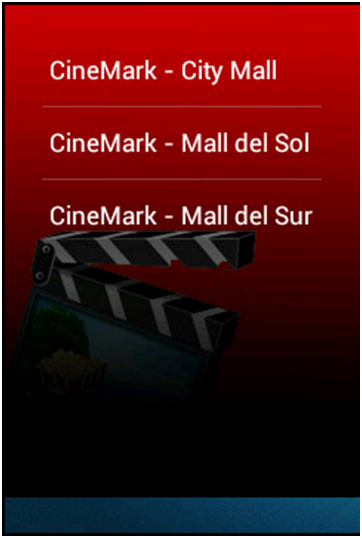
\includegraphics[totalheight=1.8in,width=1.4in]{mapas}
\end{center}







\end{document}